\chapter{Night 4: Facial Recognition, Image Manipulation and Decomposition}

\begin{learningobjectives}
\emph{Concepts}
\bi
\item Describe how a vector can be used to represent a data set.
\item Explain how a matrix is used to represent multiple data sets.
\item Explain what is meant by vectorizing a grayscale image.
\item Predict the size of a vectorized image, given its pixel dimensions and color (gray or color). 

\ei
\emph{MATLAB skills}
\bi
\item Convert a color image into a grayscale image.
\item Convert an image to a matrix and back again
\ei
\end{learningobjectives}

\section{Ethics, Artificial Intelligence, and Facial Recognition}

Face recognition is a technology with many possible applications.  In just the past dozen or so years, the technology has gone from the stuff of science fiction to something that we interact with everyday (e.g., auto-tagging of images uploaded to social media).  In this part of the assignment we are going to ask you to take a deep dive into how this technology manifests itself in the real world---often with mixed consequences for society.

This section is structured into three parts.  First, we'll have you read about some of the issues that have been raised around face recognition technology (and more generally face analysis technology).  Next, you'll read some frameworks that have been proposed to help mitigate the potential harm and maximize the benefits that might otherwise come from releasing poorly tested and biased AI systems.  Finally, we'll have you branch out from face recognition technology to AI in general to examine which applications of the technology you think have the potential to most positively impact the world.  You will discuss and synthesize your findings in class on Thursday, so make sure to take some sort of notes on what you read (there are also some specific prompts to respond to below).

\subsection{Face Recognition Technology}


\begin{prob}
For a good overview of the issues, we'd like you to read \href{https://docs.house.gov/meetings/GO/GO00/20190522/109521/HHRG-116-GO00-Wstate-BuolamwiniJ-20190522.pdf}{Joy Buolamwini's written testimony} that she then \href{https://youtu.be/jLmzEFkbNsg?t=2910}{presented orally} .  You can pick whether you read the testimony or watch the video, although one nice thing about the written testimony is that it cites a lot of sources that you can read for more information.

\emph{Based on this reading, generate a list of surprising insights (e.g., spurred by key quotes) that you gained.  Also generate at least one discussion question.}
\end{prob}

\subsection{Frameworks and Guidelines for Responsible Machine Learning}

\begin{prob}
Face recognition technology falls under the umbrella of machine learning.  Machine learning is a field concerned with creating technologies that enable computers to learn to perform tasks automatically from experience (e.g., recognizing someone's identify from a picture of their face)---often by ingesting large training sets of labeled data.  Sparked by a recognition that machine learning technologies were causing unanticipated harm in the real world, a lot of attention has been paid in recent years (both in industry and academia) to issues of fairness, accountability, and transparency.  Here are two frameworks that have been created.
\begin{itemize}
\item \href{https://www.fatml.org/resources/principles-for-accountable-algorithms}{Principles for Accountable Algorithms}
\item \href{https://cloud.google.com/inclusive-ml/}{Google's Inclusive ML}
\end{itemize}

\emph{Based on this reading, generate a list of surprising insights (e.g., spurred by key quotes) that you gained.  Also generate at least one discussion question.}

To get a sense of all of the conversations taking place around this topic, check out \href{https://facctconference.org/network/}{ACM's FAccT network of events}.
\end{prob}

\subsection{Beyond Face Recognition}

One thing that is important to mention at this point in the module is that while we are learning linear algebra and data analysis techniques within the context of face recognition, what you are learning can be applied to innumerable applications and fields of study.  Even if we just stay within the realm of artificial intelligence, what you are learning now (and will learn later in the course) is the bedrock of many AI algorithms that are used in all sorts of applications.  When learning about all of the issues that a technology like face recognition has, we find that students can sometimes have a tendency to move towards a nihilistic perspective on technology as a whole (e.g., all technology is bad / harmful).  Critiquing technology and its role and effect in society is absolutely vital for \emph{any} engineer.  However, we contend that trying to understand how technology can be developed in a way that minimizes harm while maximizing benefit (e.g., the frameworks from the previous section) or by applying technology to problems or domains that have great potential for positive impact is also crucial.  In this section, we are asking you to look into applications of image analysis (or artificial intelligence more generally) that have the potential for great positive impact on society.

\begin{prob}
Find an article or paper about an application of artificial intelligence (it could be specifically about image or face analysis, but it need not be) that you think has the potential for great positive impact on society.  Come to class ready to summarize the application and why you think it has the potential for positive impact.  Unpack the notion of positive impact by specifying what the benefits (or downsides) would be of the application and who would reap them.

If you need some inspiration, here are some starting points (we are not claiming these are necessarily unambiguously positive, but they may provide some good starting points for your search).
\begin{itemize}
\item Automated diagnosis of cancer from medical images
\item Automated, personalized education
\item Optimizing energy use with artificial intelligence (more generally ``Computational Sustainability'')
\item Sensing for driverless cars (e.g., pedestrian detection, road sign reading)
\item Recognition and reading of text in a camera feed for people who are blind
\item Automated wildlife monitoring via image analysis
\item This one is kind of cheating. Olin 2nd year Austin Vesiliza put together \href{https://www.notion.so/ML-for-Good-c0cc352c88b04e719c187c8e4a6f5887}{a list of links to AI for social good projects} that you might use for inspiration.
\end{itemize}
\end{prob}

\section{Manipulating Images with Matrices}

\begin{center}
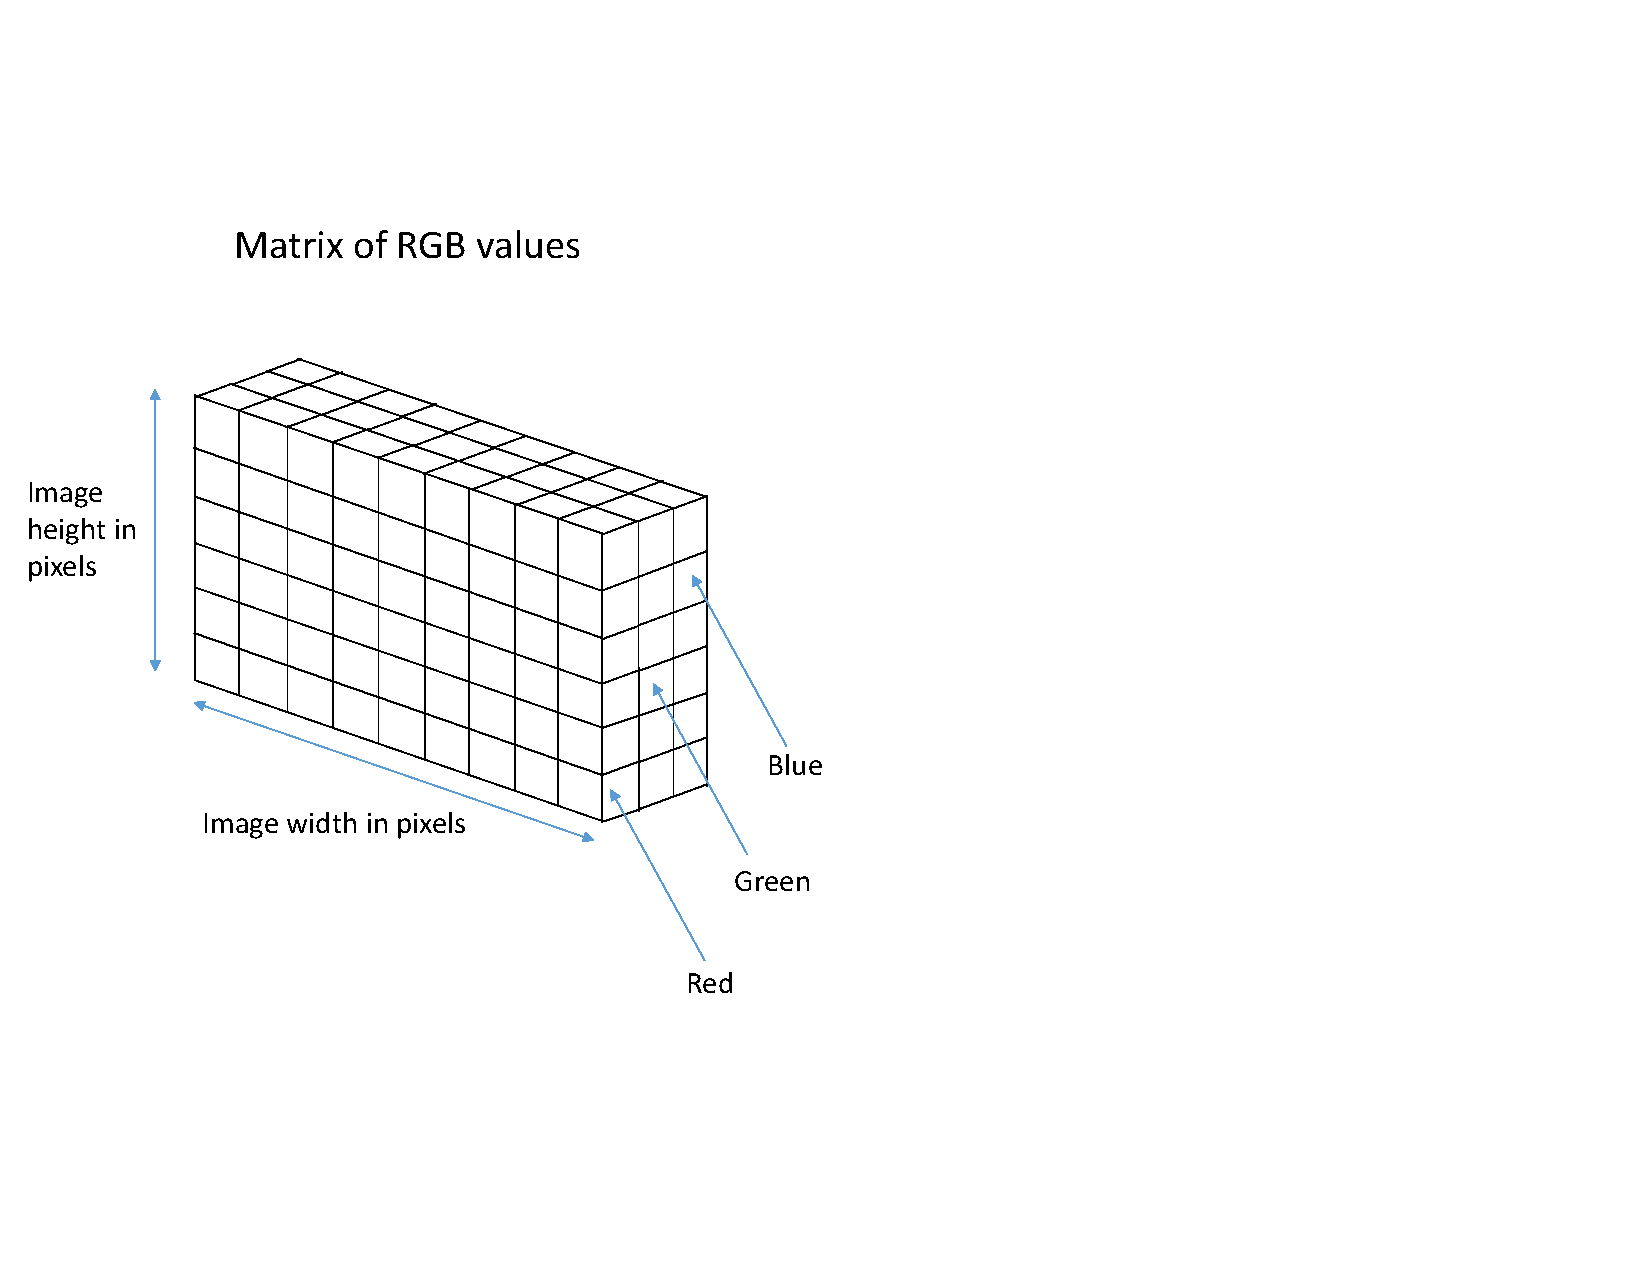
\includegraphics[width=0.75\textwidth]{FacesNight1/figs/RGBArrayWithSlice.pdf}
\captionof{figure}{Anatomy of an RGB image array.}
\label{fig:StackedRGBArray}
\label{fig:RGBArray}
\end{center}

\begin{prob}
    Our next example is of an image pre-processing step that many of you would eventually do using built-in MATLAB functions before running your face detection algorithm.
        \begin{enumerate}
        \item Read an image file using MATLAB, and convert it to double precision numbers (the data format that MATLAB uses by default for vectors and matrices) using the following code:
        \begin{verbatim}
        X = imread(`giraffe.jpg');
        \end{verbatim}
        (If you get an error, try re-typing the apostrophes.)

        \item Color images are stored in a 3-dimensional array (as opposed to matrices, which are 2-dimensional arrays) in MATLAB. Compare this to the smiley face image you saw in class which was a matrix whose entries are the gray-scale values. Here, instead of gray-scale values, the color information is stored in Red, Green and Blue entries of the three-dimensional array. Therefore, each pixel in the image is associated with three different values which indicate how much of Red, Green and Blue are present in that pixel.  This array is illustrated in Figure \ref{fig:RGBArray}.

         You can see the dimensions of this array using the following.
        \begin{verbatim}
        size(X)
        \end{verbatim}

        \item Display the image using

        \begin{verbatim}
        imagesc(X);
        \end{verbatim}

    The image may be squashed; if you would like it not be be squashed, type \texttt{axis equal} into the command window.

    \item What will the dimensions of the matrix with the grayscale representation of this image be? 
    
    \item We will now use matrix manipulations to turn the image into a grayscale image. The RGB array can be separated into three slices, one for each color. For example, the red slice is all the data in the the first layer of the array:
    \begin{verbatim}
    X_red=X(:,:,1);
    \end{verbatim}

    Converting a pixel to grayscale can be accomplished by taking a linear combination of the red, green and blue values of that pixel which are weighted by 0.2989, 0.5870 and 0.1140 respectively. Use these weights to create a linear combination of the red, green, and blue slices.


    \item  Verify if this was done correctly by displaying the image using the following commands.
    \begin{verbatim}
    imagesc(grayscaleX); colormap('gray'); axis equal
    \end{verbatim}

    \end{enumerate}
    \end{prob}
    
    \begin{sol}
    \begin{enumerate}
    \item 
        \item The size of the array is $740\times740\times3$.
        \item You should see the following picture:
            \begin{center}
            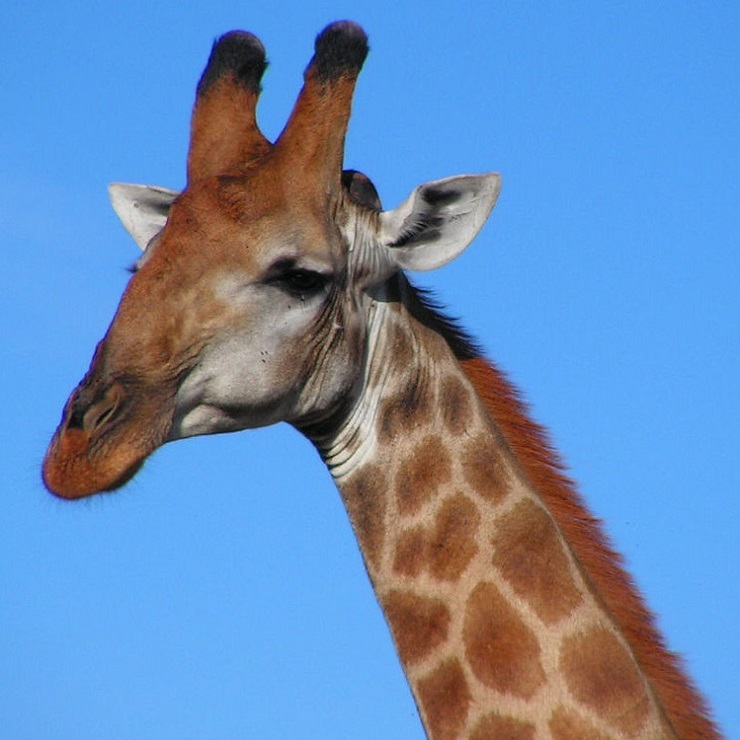
\includegraphics[scale=.4]{FacesNight1/figs/giraffe.jpg}
            \captionof{figure}{Giraffe}
            \label{fig:giraffe}
            \end{center}
        \item The gray-scale version of this image is represented by a $740\times740$ matrix.
        \item Create the matrix $\mathbf{grayscaleX}$ which represents the grayscale version of this image using \texttt{>> grayscaleX = 0.2989*X(:,:,1) + 0.5870*X(:,:,2) + 0.1140*X(:,:,3)}.
        \item You should see the following image:
                \begin{center} 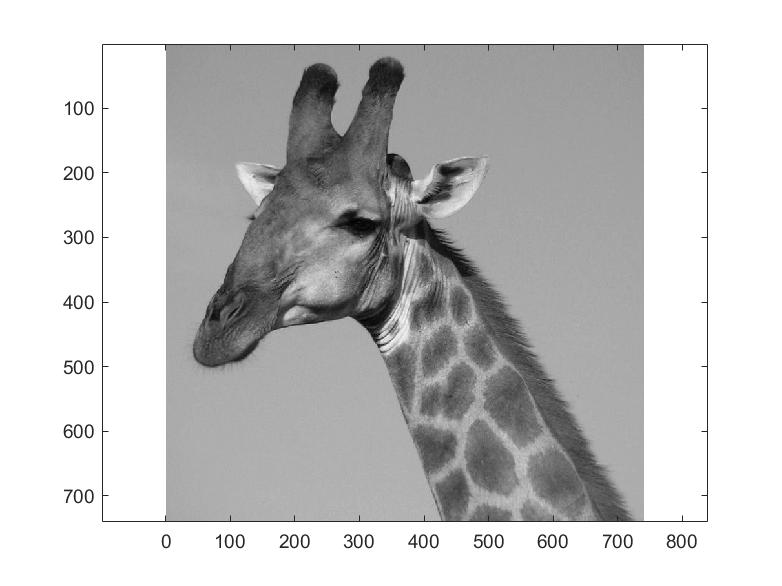
\includegraphics[scale=.4]{FacesNight1/figs/graygiraffe.jpg}
                \captionof{figure}{Gray Giraffe}
                \label{fig:graygiraffe}
                \end{center}
    \end{enumerate}
    \end{sol}

\section{Further Examples on Decomposition}


\begin{prob}
\begin{enumerate}

\item In this problem, we are going to express the temperature data for four cities we encountered earlier using a given set of basis vectors. Load some sample temperature data in MATLAB by typing \texttt{>> load  temperatures\_and\_bases.mat}. Type \texttt{whos} at the MATLAB prompt to see all your variables. You should have a matrix \texttt{T} which has the temperature data for 1 year for the cities of Boston, New York, Washington DC and Providence in that order. Use the \texttt{size} command to determine how the data are organized in this matrix. You should also have four vectors $\u_1\cdots\u_4$ which a genie has provided to you.

\begin{enumerate}

\item Verify that the vectors $\u_1, \cdots \u_4$ are all mutually orthogonal, and that they have unit length.

\item Set up and solve the linear algebra problem in order to express each column of the temperature matrix \texttt{T} as a linear combination of $\u_1\cdots\u_4$. Check that you can undo this operation and retrieve the original data.

\item Now let's reconstruct an approximation to the original temperature data, using only the vectors $\u_1, \u_2, \u_3$, What is the rms error for this approximation?

\item Compare the rms error for the previous scheme to a simpler scheme where in order to compress the data, we simply discard the temperature of Providence. When we want to reconstruct the data, we simply approximate the temperature in Providence by the temperature in Boston.

\end{enumerate}

Once again, we have to disappoint you by letting you know that there is no genie! There is just data. In the coming weeks, we are going to find out how to find bases vectors that can be useful for dimensionality reduction for a given set of random data, given some training data. This will be particularly useful in speeding up computations where instead of doing computations on all the dimensions of the data we have, we perform computations on fewer dimensions.

\item We will finally be dealing with images of faces. We are going to compress these face images in a similar way as the temperature data (we give you the bases). Here, the data have really high dimensions (each pixel is a dimension). The bases that we give you (matrix $\mathbf{U}$) doesn't span the entire high dimensional space (so there will be lossy compression).

\begin{enumerate}

\item Load the file \texttt{face\_bases.mat} in MATLAB. You will see a 3-dimensional array \texttt{test\_images}, of dimensions $256\times 256\times 424$, and a matrix \texttt{U} of dimensions $65536 \times 424$. The \texttt{test\_images} array contains 424 grayscale images.Each image is $256 \times 256$ pixels.

\item Select any one image from the set of 424 and call it \texttt{T}. Display this image using \texttt{>> imagesc(T); colormap('gray')}. This image is currently represented as a $256 \times 256$ matrix of grayscale values. We will find it very convenient to work with vectors instead of matrices representing an image. Therefore, to make our lives simple, we will take the data for an image which is stored in a matrix and store it in a vector.

We are going to \emph{vectorize} this image by stacking its columns one on top of another to create a single vector that is $(256)^2 \times 1$, i.e. $65536 \times 1$ which will be a lot easier to work with. This operation can be accomplished in MATLAB as follows: \texttt{>> Tstacked = reshape(T, 65536,1);}. When you need to recover the unstacked version of the image, you can undo-the stacking as follows: \texttt{>> Tunstacked = reshape(Tstacked, 256, 256)}.

\item The matrix \texttt{U} contains a set of 424 $65536 \times 1$ linearly independent vectors provided by the genie. Approximate the \texttt{Tstacked} vector as a linear combination of the first $10$ of columns of \texttt{U}, and call this vector \texttt{Tapprox10}. \texttt{Tapprox10} should be a 65536 $\times$ 1 vector, and you will only have 10 weight values to find this approximation. See how well this approximation works by reshaping \texttt{Tapprox10} into a $256 \times 256$ matrix and displaying it using \texttt{imagesc} and \texttt{colormap('gray')}.

\item Now repeat the previous exercise with the first 50 columns of \texttt{U} and then again with the first 100 columns of \texttt{U}. 

\end{enumerate}

You should observe that the more columns of \texttt{U} you use, the better the approximation. Note here that we are trying to approximate a 65536 dimensional vector using 10, 50 and 100 numbers. Therefore, you should not expect the approximation to work super well, but with 100 columns of \texttt{U}, you should be able to recognize the picture. At a later date we will quantify the fidelity of the approximation.

Note that more sophisticated image compression algorithms use methods that rely on special properties of images and human vision in order to a achieve high degree of compression.

\end{enumerate}
\end{prob}
\begin{sol}
\begin{enumerate}
    \item \begin{enumerate}
        \item To check that \texttt{u1} and \texttt{u2} are orthogonal, type \texttt{>> transpose(u1)*u2}. The result should be zero. Check the other five pairs of vectors.
        
        To check that \texttt{u1} has unit length, type \texttt{>> transpose(u1)*u1}. The result should be one. Check the other three vectors.
        
        \item First we need to construct a matrix \texttt{U} with columns each of the $\mathbf{u}_i$\\
        \texttt{>> U=[u1 u2 u3 u4],}\\
        and convert \texttt{T} to the basis of $\mathbf{u}_i$ vectors by multiplying
        \texttt{>> Tu=U*T.} You can recover the original data with \texttt{>> inv(U)*Tu}.
        
        \item 
        \item
    \end{enumerate}
    \item \begin{enumerate}
        \item 
        \item
        \item Isolate the first 10 columns of \texttt{U} using \texttt{>> U10=U(:,1:10);}. Then determine the weights for each of these column vectors using\\
        \texttt{>> Tweights10=transpose(Tstacked)*U10;}\\
        and then take the linear combination\\
        \texttt{>> Tapprox10=U10*transpose(Tweights10);.}
        Then we unstack the vector into a matrix\\
        \texttt{>> Tapprox10unstacked=reshape(Tapprox10,256,256);}
        and display the image.
        \item 
    \end{enumerate}
\end{enumerate}
\end{sol}

% \subsection{Check in with your concept map}

% \begin{prob}

% Pull up the picture of your concept map of eigenfaces from the first day of this module.  Annotate this picture (in whatever way you prefer) to indicate where we have gotten so far in this.  Add additional bubbles or nodes to the concept map if there are things we have learned up to this point that were not in your original!  Also annotate your concept map as to which things we still need to learn to get all the way to eigenfaces.

% \end{prob}

\section{Data: Many Measurements of the Same Thing}
{One of the simplest forms of data} is a set of data which represents many measurements of nominally the same thing.  Depending on what the goal is of our analysis, this might encompass measurements of the same quantity across many different situations, or many instances of the same situation.
\subsection{Visualizing Measurements of the Same Thing}

It's usually a good idea to \textit{look} at data before you start calculating things associated with it.

You've surely encountered these ideas before, but for the sake of completeness, we'll highlight a couple of ideas here.  If you have a large number of data points (say, for example, that you measured the heights of a bunch of different people), you might choose to simply plot the data versus the person number -- the index.  Note here that the data is plotted as individual points, since each point represents a measurement.  Ideally we might also include error bars here to indicate our uncertainty in a given measurement, but for now, let's leave that out.

\begin{center}
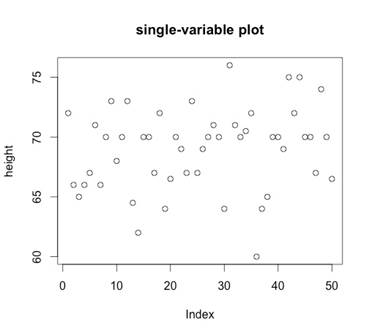
\includegraphics[width=0.75\textwidth]{FacesNight3/figs/singlevariableplot.jpg}
\captionof{figure}{An example of a single variable plot}
\label{fig:single-var-plot}
\end{center}

Alternatively, you could also visualize many measurements of the same thing by creating a \textit{histogram}.  This is a representation of how many measurements fall into different ``bins'': the height of a given bar is the number of samples that fall within the range associated with the bar.  For example, in the figure, you can see that about 20 million people made between 0 and \$5000 in 2008.  You've likely seen this kind of thing before as well: it's not an uncommon way to represent test scores.

\begin{center}
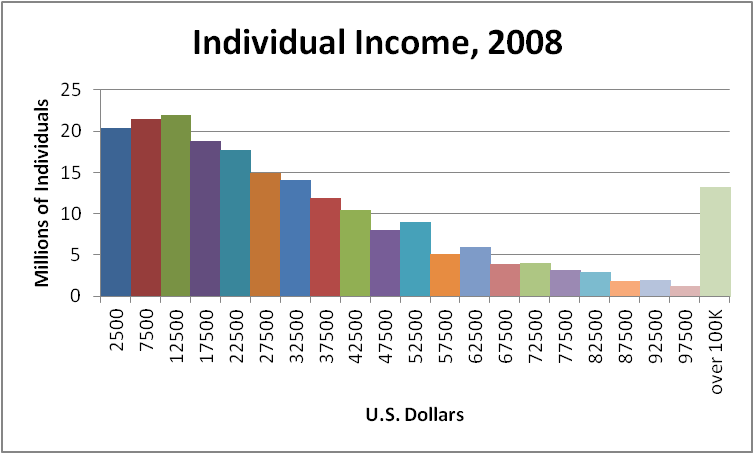
\includegraphics[width=0.75\textwidth]{FacesNight3/figs/incomehistogram.png}
\captionof{figure}{An example of a histogram.}
\label{fig:histogram}
\end{center}

Note, of course, that how a histogram \textit{looks} depends on what you choose for the bins - both how many there are, and where they are centered!

\subsection{Common Figures of Merit for the Same Thing }
While looking at the data is certainly helpful, we can also extract or calculate a couple of important figures of merit of the data.  The first is the average, or \textit{mean} of the data, given by summing all the elements in the dataset $\{d_i\}$ and dividing by the number $N$ of elements in the set:
\begin{equation}
\mu  =  \frac{1}{N}\sum_{i=1}^N d_i
\end{equation}
Note that if our data is a continuous function $f(x)$ over a range of the independent variable $x$ as opposed to a set of discrete points, we can express the same thing as an integral:
\begin{equation}
\mu = \frac{\int_{range} f(x) dx}{\int_{range} dx}
\end{equation}
The average captures the center or 'expected value' of the distribution of data.  In addition to this, it is often helpful to capture the spread of the data around this average.  There are a few different metrics which are used for this.  A simple one is the \textit{variance} from the mean, $\sigma^2$:  the average of the squared difference between each data point and the mean.
 \begin{equation}
\sigma^2  =  \frac{1}{N-1}\sum_{i=1}^N (d_i - \mu)^2
\end{equation}
Please note that this definition normalizes using $N-1$, but you will often see alternative definitions which normalize using $N$. Another commonly encountered measure is the \textit{standard deviation}, which is simply the square root of the variance from the mean:
 \begin{equation}
\sigma  =  \sqrt{\frac{1}{N-1}\sum_{i=1}^N (d_i - \mu)^2}
\end{equation}

\begin{prob}
\begin{enumerate}
\item Look at the single variable plot in Figure~\ref{fig:single-var-plot} above.  Estimate the value of the mean and the value of the standard deviation.  What are the units of each?
\item Look at the histogram plot in Figure~\ref{fig:histogram} above.  Estimate the value of the mean and the value of the standard deviation.
\item What is the mean and standard deviation of this data set (Do this in your head!)
$$\{1,3,1,3,1,3,1,3,1,3,1,3,1,3,1,3,1,3,1,3\}$$
\item  Begin by considering the simple dataset of the high temperatures in Needham for ten days in March:
\begin{equation}
T = \{57,61,46,43,46,46,54,46,46,55\}
\end{equation}
\begin{enumerate}
\item  By hand, create a histogram of this data.  What size bin makes sense? What bin centering makes sense?
\item  By hand, compute the mean temperature over these ten days.  If you look at the data, does this mean make sense?
\item  By hand, compute the variance and standard deviation of the temperature over these ten days.  If you look at the data histogram does this make sense?
\item  This dataset has a flaw: it has a small number of datapoints.  What do you see as the possible effects of having such a small sample?
\end{enumerate}
\item  Now consider the larger dataset below of the approximated heights of the Olin faculty, measured in inches.  In MATLAB, create a vector which has this dataset as the entries.
\begin{align*}
H = &\{63,66,71,65,70,66,67,65,67,74,64,75,68,67,70,73,66,70,72,62,68,\\
&70,62,69,66,70,70,68,69,70,71,65,64,71,64,78,69,70,65,66,72,64\}
\end{align*}
\begin{enumerate}
\item  Computationally histogram this data.  What size bin makes sense?  What bin centering makes sense? Try a few different combinations. See MATLAB function \texttt{histogram}.
\item  Computationally, find the mean, standard deviation, and variance of this dataset. See MATLAB functions \texttt{mean}, \texttt{std}, and \texttt{var}.
\item  Does the mean, standard deviation, and variance make sense given the histogram of the data?
\end{enumerate}
\end{enumerate}
\end{prob}
\begin{sol}
\begin{enumerate}
    \item Assuming that the ``heights'' plotted are heights of randomly selected humans, then the unit for the mean and standard deviation is inches.
    \item 
    \item Since half the digits are 1 and the other half are 3, the mean will be the average of 1 and 3, so $\mu=2$. Looking at the formula for standard deviation, we can see that $d_i-\mu = 1$ for each data point, so $\sigma = \sqrt{20/19}$.
    \item \begin{enumerate}
        \item 
        \item We compute $\mu=50$.
        \item We compute $\sigma=6.15$.
        \item 
    \end{enumerate}
    \item 
    \begin{enumerate}
        \item By simply entering \texttt{>> histogram(H)}, MATLAB automatically chooses bins of size one.
    \item Using MATLAB we find that $\mu = 68.1429$, $\sigma = 3.5721$ and $\sigma^2 = 12.7596$.
    \item 
    \end{enumerate}
\end{enumerate}
\end{sol}


\section{Brightness and Contrast}
The brightness and contrast of images is controlled by scaling the histogram of the pixel values.  Try this out!

Note:  for displaying images in this part, make sure to NOT use imagesc:  imagesc is specifically setup to auto-scale the image to use the full range from 0 to 255. Just use the command `image'.

\begin{prob}
    \begin{enumerate}
    \item  Load an image of your choice into MATLAB using the \texttt{imread} command.  (Make sure you are in the correct directory for the image or give it the complete path). Display the image using the `image' command.
    \item  If your image is a color image, convert it into grayscale by using the \texttt{rgb2gray} command.
    \item  Create a vector of the intensities in your image: use the \texttt{reshape} command to create a giant column vector in which the first $n$ elements are the first column of the image, the next $n$ are the second column, etc.
    \item Make a histogram of the intensity values in your image.  Note that the default variable type for image data is uint8 (8-bit unsigned integer) which is an integer that ranges from 0 to 255.   Does your image use the entire range of values from 0 to 255?  What is the minimum pixel value used?  What is the maximum?
    \item  Find the mean of the intensities in your image data.  Find the standard deviation.  Is the intensity data well-centered on the available range?  The location of the intensity data in the range determines the brightness of the image. How does the standard deviation compare to the available range?  Does the intensity data span a good portion of the available range? This affects the contrast.
    \item  To adjust the brightness of your image, you can scale all of the intensity values by a multiplicative factor down (towards darker values) or up (towards brighter values).  Based on looking at the histogram, should your image be brightened?  Dimmed?  Why?
 \item To adjust the contrast, you make a linear mapping of the existing range onto the full 0 to 255 range.  In other words, if you think of the current intensity value as your independent variable $x$, and the new intensity value as the dependent variable $y$, a contrast adjustment is defined by a function $y = f(x)$.  Propose an equation for a line which gives you the ``best'' range of y's, given the input intensity values in the image.  You should be able to justify this based on the histogram of the image.  Note that any values  of $y$ that end up below 0 should be interpreted as 0, and any values over $255$ should be interpreted as $255$.
 \item Implement brightness and contrast adjustment:
 \begin{enumerate}
 \item Load a picture of a face.
 \item Analyze the intensity histogram.
 \item Calculate the adjusted face by applying both brightness and contrast adjustments to make it as ``good'' as possible.
 \item Create a figure that includes four subplots: the original image, the original intensity histogram, the new image, and the new intensity histogram.
 \end{enumerate}
 \item What would happen if the function for contrast adjustment was not linear?  Why might you choose a non-linear function for this mapping?
 \end{enumerate}
\end{prob}

\pagebreak
\shipoutAnswer
